\chapter[Extensibility and Spatial Chaos]{Spatial Chaos in Extensible Rods in a Uniform Magnetic Field} \label{chap:analytical}
%
In this chapter the noncanonical equilibrium equations for a rod in a magnetic field are reduced on the symplectic leaves determined by the three Casimirs using Euler angles. From this reduction two principles are illustrated; firstly the integrability of an linearly elastic, isotropic, inextensible unshearable rod in a uniform magnetic field is shown and secondly it is shown, through Mel'nikov analysis, that when the rod is extensible it is no longer integrable. In the integrable case the reduction gives a four-dimensional canonical system with a first integral and a Hamiltonian. By specifying an energy level that constrains the orbits to a surface in three-dimensions, Poincar\'e sections yield closed curves. For an extensible rod it is then shown that the magnetic field destroys complete integrability through the loss of a first integral and Smale horseshoes are shown to exist on the Poincar\'e section of the homoclinic energy level, in direct contrast to the regular dynamics illustrated in the integrable case. 
% 
\section{Reformulation} \label{sec:reform}
% 
For clarity when describing the family of rod models, in~\S\ref{chap:model} the governing equation for rod in a uniform magnetic field was presented in terms of three field variables $\mathsf{m}$, $\mathsf{n}$ and $\mathsf{B}$. However, in order to apply a suitable perturbation it is necessary to express the magnetic field in terms of the unit vector $\mathsf{e}_{3}$ and a bifurcation parameter $\lambda$, following Wolfe's notation~\cite{Wolfe83,Wolfe85,Wolfe88,Wolfe90a,Wolfe90b,Wolfe96}, such that $\mathsf{B} = \lambda \mathsf{e}_{3}$ where $\lambda = IB$. Thus the governing equations can be expressed as
%
\begin{align}
\left( \begin{array}{c}
\mathsf{m} \\
\mathsf{n} \\
\mathsf{e}_{3} 
\end{array}
\right)^{\prime} & = 
\left( \begin{array}{ccc}
\hat{\mathsf{m}} & \hat{\mathsf{n}} & \hat{\mathsf{e}}_{3} \\
\hat{\mathsf{n}} & \lambda \hat{\mathsf{e}}_{3} & \mathsf{0} \\
\hat{\mathsf{e}}_{3} & \mathsf{0} & \mathsf{0} 
\end{array} \right)
\left( \begin{array}{c}
\mathsf{u} \\
\mathsf{v} \\
\mathsf{0} 
\end{array}
\right).
\end{align}
% 
The Casimirs of the system are then given by
% 
\begin{subequations}
\begin{align}
C_{1} & = \frac{1}{2}\mathsf{n}\cdot\mathsf{n} + \lambda \mathsf{m}\cdot\mathsf{e}_{3}, \label{eq:mag_casimir1} \\
C_{2} & = \mathsf{n}\cdot\mathsf{e}_{3}, \label{eq:mag_casimir2} \\
C_{3} & = \mathsf{e}_{3}\cdot\mathsf{e}_{3}.\label{eq:mag_casimir3}
\end{align}
\end{subequations}
% 
The integrals, conditionally dependent on $B=B_{1}=B_{2}$ and $J=K=H=0$, are given by
% 
\begin{subequations}
\begin{align}
I_{1} & = m_{3}, \\
I_{2} & = \mathsf{m}\cdot\mathsf{n} + B\lambda e_{33}.
\end{align}
\end{subequations}
%
Now the nondegeneracy condition states $C_{3} \ne 0$. Note that the Casimir~\eqref{eq:mag_casimir1} now features the parameter $\lambda$.
%  
\section{Reduction to a Canonical System} \label{sec:reduction}
%
In this section the three Casimirs~\eqref{eq:magnetic_casimirs} are used to reduce the nine-dimensional non-canonical Hamiltonian system~\eqref{eq:magnetic_equations} to a six-dimensional canonical Hamiltonian system using Euler angles. This is possible (at least locally) provided the structure matrix~\eqref{eq:magnetic_structure} is of constant rank everywhere~\cite[\S{6.2}]{Olver93}. The reduction is performed by constructing a coordinate transformation from the nine coordinates $\left(\mathsf{m},\mathsf{n},\mathsf{e}_{3}\right)$ to three Euler angles $q=\left(\theta,\psi,\phi\right)$ and their canonical momenta $p=\left(p_\theta,p_\psi,p_\phi\right)$.  The reduction follows~\cite{Thiffeault01} but here the system is shown to be canonical. As it happens, the transformation is only canonical subject to a non-alignment condition. The aligned case is also of interest and is treated in~\S\ref{subsec:alignment}. 
%
\par
Assuming, without loss of generality, that
%
\begin{align}
\mathsf{e}_{3}\left(q\right) & = R\left(q\right) k = 
\left(
\begin{array}{c}
-\sin\theta\cos\phi\\
\sin\theta\sin\phi\\
\cos\theta
\end{array}
\right),
\label{eq:canonical_magnetic}
\end{align}
%
where $k=\left(0,0,1\right)^T$ and $R\left(q\right)$ is given by~\eqref{eq:euler_matrix}.
%
\par
On inserting the Euler angles into the strains~\eqref{eq:curvatures} and using the constitutive relations~\eqref{eq:constit} and the orthornormality of the directors, the moments are parametrised by~\eqref{eq:noncanonical_moment1}
% 
\begin{subequations}
\begin{align}
m_{1} & = p_{\theta}\sin\phi - \cos\phi \left( \frac{p_{\psi} - p_{\phi}\cos\theta}{\sin\theta} \right),\nonumber \\
m_{2} & = p_{\theta}\cos\phi + \sin\phi \left( \frac{p_{\psi} - p_{\phi}\cos\theta}{\sin\theta} \right),\nonumber\\
m_{3} & = p_{\phi}. \nonumber 
\end{align}
\end{subequations}
% 
The moments can be expressed in the compact matrix form as $\mathsf{m} = Lp$ (see~\eqref{eq:noncanonical_moment}). Finally, the force may be written as
%
\begin{align}
\mathsf{n}\left( q,p \right) & = R\left(q\right)v\left(q,p\right), \nonumber
\end{align}
%
for some non-constant triple $v$. Decomposing $v$ as
%
\begin{align}
v\left(q,p\right) & = v_{\perp}\left(q,p\right) {i}_{\perp} + v_{\parallel}\left(q,p\right) {i}_{\parallel}, \nonumber
\end{align}
%
where ${i}_{\parallel}$ and ${i}_{\perp}$ are unit triples parallel and perpendicular to $k$, respectively. Thus~\eqref{eq:mag_casimir2} yields
%
\begin{align}
C_{2} & = \mathsf{n}\cdot\mathsf{e}_{3} =  R k \cdot R v = v \cdot \left( R^{T} R \right) k = v_{\parallel}.
\end{align}
%
Furthermore, from~\eqref{eq:mag_casimir3}
%
\begin{align}
C_{1} & = \frac{1}{2}R v\cdot Rv + \lambda L p \cdot R k = \frac{C_{2}^{2}}{2} + \frac{1}{2}v_{\perp}^{2} + \lambda p \cdot \left( L R^{T} \right) k,
\end{align}
%
which allows us to solve for $v_{\perp}$:
%
\begin{align}
v_{\perp}\left( q,p \right) & = \sqrt{ 2C_{1}^{} - C_{2}^{2} - 2 \lambda p \cdot \left( L R^{T} \right) k} =
\sqrt{ 2C_{1}^{} - C_{2}^{2} - 2 \lambda p_{\psi}^{} },
\label{eq:handedness}
\end{align}
%
where, without loss of generality, the positive solution is taken. If the vector perpendicular to $k$ is taken to be $i_{\perp} = \left( 1,0,0 \right)^T$ then
%
\begin{align}
\mathsf{n} & = 
C_{2}^{}
\left( \begin{array}{c}
-\sin\theta\cos\phi \\
\sin\theta\sin\phi \\
\cos\theta
\end{array} \right) \nonumber \\
& \hspace{1.0cm}
+ \sqrt{ 2C_{1}^{} - C_{2}^{2} - 2 \lambda p_{\psi}^{}  }
\left(\begin{array}{c}
 \cos\theta\cos\phi\cos\psi-\sin\phi\sin\psi \\
-\cos\theta\sin\phi\cos\psi-\cos\phi\sin\psi \\
 \sin\theta\cos\psi
\end{array}
\right). \label{eq:canonical_force}
\end{align}
%
Note that this transformation is well-defined as 
% 
\begin{align}
2C_{1}^{} - C_{2}^{2} - 2 \lambda p_{\psi}^{} & = v_{\perp}^{2} \ge 0. \label{eq:alignment_condition}
\end{align}
%
\par
In contrast to the reduction of the Kirchhoff equations, the equations~\eqref{eq:canonical_magnetic},~\eqref{eq:noncanonical_moment1} and~\eqref{eq:canonical_force} give a representation of the three field variables in terms of all of the the Euler angles. In order for the bracket noncanonical~\eqref{eq:magnetic_bracket} to be transformed to canonical form for the Euler angles it is necessary to verify that
%
\begin{align}
G \mathcal{J} G^{T} & = \bar{\mathcal{J}}, \nonumber
\end{align}
%
where $\mathcal{J}$ is the structure matrix defined in~\eqref{eq:magnetic_structure} and $\bar{\mathcal{J}}$ is the standard canonical structure matrix in $\mathbb{R}^{6}$ and the $G$ is the Jacobian matrix
%
\begin{align}
G & = \frac{ \partial \left( q, p \right) }{ \partial \left( \mathsf{m}, \mathsf{n}, \mathsf{e}_{3} \right) }.
\label{eq:G}
\end{align}
% 
Expressing the new canonical variables by inverting the non-canonical variables~\eqref{eq:canonical_magnetic},~\eqref{eq:noncanonical_moment1} and~\eqref{eq:canonical_force} yields
%
\begin{align}
\theta & = \cos^{-1} e_{33}^{}, \nonumber \\
p_{\theta} & =  \frac{m_{1}e_{32}-m_{2}e_{31}}{\sqrt{1-e_{33}^{2}}}, \nonumber \\
\phi & = \tan^{-1}\frac{ -e_{32} }{ e_{31} }, \nonumber \\
p_{\phi} & = m_{3}, \nonumber \\
%
\psi & = \cos^{-1} \left( \frac{ n_{3}^{}-C_{2}^{}e_{33}^{} }{ \sqrt{\left(1-e_{33}^{2}\right)\left(2C_{1}^{}-C_{2}^{2}-2\lambda\left(m_{1}^{}e_{31}^{}+m_{2}^{}e_{32}^{}+m_{3}^{}e_{33}^{}\right)\right)} } \right), \nonumber \\
%
p_{\psi} & = \left( m_{1}e_{31}+m_{2}e_{32}+m_{3}e_{33}\right). \nonumber
\end{align} 
%
Explicitly, the transformation matrix $G$ is given by
%
\begin{align} 
G & = \left( 
\begin{array}{ccccccccc}
0 & 0 & 0 & 0 & 0 & 0 & 0 & 0 & -\sqrt{ \frac{1}{1-e_{33}^{2}} } \\  
0 & 0 & 0 & 0 & 0 & 0 & \frac{e_{32}^{}}{e_{31}^{2}+e_{32}^{2}} & \frac{-e_{31}^{}}{e_{31}^{2}+e_{32}^{2}} & 0 \\ 
g_{31} & g_{32} & g_{33} & g_{34} & g_{35} & g_{36} & g_{37} & g_{38} & g_{39} \\ 
\frac{e_{32}^{}}{\sqrt{1-e_{33}^{2}}} & \frac{-e_{31}}{\sqrt{1-e_{33}^{2}}} & 0 & 0 & 0 & 0 & \frac{-m_{2}}{\sqrt{1-e_{33}^{2}}} & \frac{m_{1}}{\sqrt{1-e_{33}^{2}}} & \frac{\left(m_{1}^{}e_{32}^{}-m_{2}e_{31}\right)e_{33}^{}}{\left(1-e_{33}^{2}\right)^{3\slash2}} \\ 
0 & 0 & 1 & 0 & 0 & 0 & 0 & 0 & 0 \\ 
e_{31}^{} & e_{32}^{} & e_{33}^{} & 0 & 0 & 0 & m_{1} & m_{2} & m_{3}
\end{array} 
\right), \nonumber
\end{align}
%
where
%
\begin{align}
g_{31} & = -\frac{ e_{31}\left( n_{3}-C_{2}e_{33} \right)}{ \Delta }, \nonumber \\
g_{32} & = -\frac{ e_{32}\left( n_{3}-C_{2}e_{33} \right)}{ \Delta }, \nonumber \\
g_{33} & = -\frac{ e_{33}\left( n_{3}-C_{2}e_{33} \right)}{ \Delta }, \nonumber \\
g_{34} & = 0, \nonumber \\
g_{35} & = 0, \nonumber \\
g_{36} & = -\frac{ 1 }{ \Delta }, \nonumber \\
g_{37} & = -\frac{ m_{1}\left( n_{3}-C_{2}e_{33} \right)}{ \Delta }, \nonumber \\
g_{38} & = -\frac{ m_{2}\left( n_{3}-C_{2}e_{33} \right)}{ \Delta }, \nonumber \\
%
g_{39} & = \frac{ C_{2}\left(2C_{1}^{}-C_{2}^{2} - 2\lambda\mathsf{m}\cdot\mathsf{e}_{3}\right) }{ \Delta }, \nonumber \\
& \hspace{1.0cm} - \frac{ \left(n_{3}-C_{2}e_{33}\right)\left( e_{33}\left(2C_{1}-C_{2}^{2}-2\lambda\mathsf{m}\cdot\mathsf{e}_{3}\right)-m_{3}\left(1-e_{33}\slash{C_{2}} \right) \right) }{ \Delta } . \nonumber 
\end{align}
%
with the denominator given by
%
\begin{align}
\Delta & = \left( 2C_{1}^{} - C_{2}^{2} - 2\lambda\mathsf{m}\cdot\mathsf{e}_{3} \right) \sqrt{ \left(1-e_{33}^{2}\right)\left( 2C_{1}^{}-C_{2}^{2}-2\lambda\mathsf{m}\cdot\mathsf{e}_{3} \right) - \left(n_{3}^{}-C_{2}^{}e_{33}^{}\right)^{2} }. \nonumber 
\end{align}
%
The non-canonical structure matrix is given by 
%
\begin{align}
\mathcal{J} & = \left( 
\begin{array}{cccccccccc}
0 & -m_{3} & m_{2} & 0 & -n_{3} & n_{2} & 0 & -e_{33} & e_{32} \\
m_{3} & 0 & -m_{1} & n_{3} & 0 & -n_{1} & e_{33} & 0 & -e_{31} \\
-m_{2} & m_{1} & 0 & -n_{2} & n_{1} & 0 & -e_{32} & e_{31} & 0\\
0 & -n_{3} & n_{2} & 0 & - e_{33} & e_{32} & 0 & 0 & 0 \\
n_{3} & 0 & -n_{1} & e_{33} & 0 & -e_{31} & 0 & 0 & 0 \\
-n_{2} & n_{1} & 0 & -e_{32} & e_{31} & 0 & 0 & 0 & 0 \\
0 & -e_{33} & e_{32} & 0 & 0 & 0 & 0 & 0 & 0\\
e_{33} & 0 & -e_{31} & 0 & 0 & 0 & 0 & 0 & 0\\
-e_{32} & e_{31} & 0 & 0 & 0 & 0 & 0 & 0 & 0
\end{array}
\right), \nonumber
\end{align}
%
while the canonical structure matrix is given by
%
\begin{align}
\bar{\mathcal{J}} & = \left( 
\begin{array}{ccccccc}
0 & 0 & 0 & 1 & 0 & 0 \\
0 & 0 & 0 & 0 & 1 & 0 \\
0 & 0 & 0 & 0 & 0 & 1 \\
-1 & 0 & 0 & 0 & 0 & 0 \\
0 & -1 & 0 & 0 & 0 & 0 \\
0 & 0 & -1 & 0 & 0 & 0 
\end{array}
\right). \nonumber
\end{align}
% 
Thus the transformation is proper {\em provided} that $v_{\perp}>0$, i.e., provided that $\mathsf{n}$ and $\mathsf{e}_{3}$ are not aligned. Without this condition the necessary inverse transformation does not exist. Note that $\mathsf{n}$ and $\mathsf{e}_{3}$ are aligned if and only if 
% 
\begin{align}
2 C_{1}^{} - C_{2}^{2} & = 2 \lambda \mathsf{m}\cdot\mathsf{e}_{3}. 
\end{align}
% 
Now from~\eqref{eq:magnetic_casimirs1},~\eqref{eq:magnetic_force} and the conservation of~\eqref{eq:mag_casimir1} that
%
\begin{align}
2\lambda\frac{\mbox d}{\mbox{d}s}(\mathsf{m}\cdot\mathsf{e}_{3})=-\frac{\mbox d}{\mbox{d}s}(\mathsf{n}\cdot\mathsf{n})=2\mathsf{d}_3\cdot(\mathsf{e}_{3}\times\mathsf{n}),
\label{eq:align}
\end{align}
%
which vanishes if $\mathsf{n}$ and $\mathsf{e}_{3}$ are aligned. Thus the alignment condition is well defined: \emph{if the force and the magnetic field are aligned anywhere they are aligned everywhere along the rod}. As remark~\ref{rem:homoclinic} states, the alignment condition does not prohibit the existence of homoclinic orbits. 
%
% \par
% The Hamiltonian~\eqref{eq:magnetic_ham} is transformed to
% %
% \begin{align}
% \mathcal{H} & = \frac{1}{2K_1K_2\sin^2\theta}\left[ p_\theta^2\,\sin^2\theta\,(K_2-
% (K_2-K_1)\cos^2\phi)+p_\psi^2\,(K_1\sin^2\phi+K_2\cos^2\phi) \right. \nonumber \\
% & + p_\phi^2\left(\cos^2\theta\,(K_1\sin^2\phi+K_2\cos^2\phi) +(K_1K_2/K_3)\sin^2\theta\right) \nonumber \\
% & + 2(K_2-K_1)p_\theta p_\phi\sin\theta\cos\theta\sin\phi\cos\phi - 2(K_2-K_1)p_\theta p_\psi\sin\theta\sin\phi\cos\phi \nonumber \\
% & \left. - 2p_\psi p_\phi\cos\theta\left(K_1\sin^2\phi+K_2\cos^2\phi\right)
% \right] \nonumber \\
% & + C_{2}^{} \cos\theta + \sin\theta\cos\psi \sqrt{ 2C_{1}^{} - C_{2}^{2} - 2 \lambda p_{\psi}^{} }. \label{eq:ham_canon} 
% \end{align}
%
% Note that the effect of the magnetic field, which previously was encoded in the Casimirs has now been transferred to the Hamiltonian. Also note that the limit $C_3\to 0$ is singular, as was also observed in~\cite{Thiffeault01}.
%
\subsection{The Isotropic Case} \label{subsec:isotropic}
%
In the isotropic case ($B:=B_1=B_2$) the Hamiltonian~\eqref{eq:magnetic_ham} reduces to
%
\begin{align}
\mathcal{H} & = \frac{p_{\theta}^{2}}{2 B} + \frac{ \left( p_{\psi}^{}-p_{\phi}^{}\cos\theta \right)^{2} }{2 B \sin^{2}\theta} + \frac{1}{2 C}p_{\phi}^{2} +  C_{2}^{}\cos\theta  \nonumber \\
& \hspace{3.50cm} + \sin\theta\cos\psi \sqrt{ 2C_{1}^{} - C_{2}^{2} - 2 \lambda p_{\psi}^{} }. \label{eq:Euler_Ham}
\end{align}
%
Since this Hamiltonian does not depend on the angle $\phi$ the momentum $p_\phi=m_3$ is a constant. The isotropic Hamiltonian still has the $S^{1}$ symmetry. Note that the effect of the magnetic field, which previously was encoded in the Casimirs has now been transferred to the Hamiltonian. 
% Also note that the limit $C_3\to 0$ is singular, as was also observed in~\cite{Thiffeault01}.
%
\par
The additional integral~\eqref{eq:int2} in canonical variables reads
%
\begin{align}
\mathcal{I} & = \lambda B \cos\theta + C_{2}^{} p_{\psi}  \nonumber \\
& \hspace{0.5cm} - \sqrt{ 2C_{1}^{} - C_{2}^{2} - 2 \lambda p_{\psi}^{} } \left( p_{\theta}\sin\psi - \cos\psi \left( \frac{p_{\phi} - p_{\psi}\cos\theta}{\sin\theta} \right) \right),
\label{eq:constraint}
\end{align}
%
rendering the system completely integrable.
%
\par
Hamilton's equations are
%
\begin{subequations}
\label{eq:all}
\begin{align}
{\theta}^{\prime}  & = \frac{p_{\theta}}{B}, \label{eq:ham3} \\ 
{\psi}^{\prime}  & =  \frac{ \left( p_{\psi} - p_{\phi} \cos\theta \right) }{ B \sin^{2}\theta }
- \frac{ \lambda\cos\psi\sin\theta }{ \sqrt{2C_{1}^{} - C_{2}^{2} - 2 \lambda p_{\psi}^{} } }, \label{eq:ham4} \\
{p}_{\theta}^{\prime} & = \frac{\left( p_{\psi}^{}\cos\theta - p_{\phi}^{} \right)\left( p_{\psi}^{} - p_{\phi}^{}\cos\theta \right)}{ B \sin^{3}\theta } + C_{2}^{} \sin\theta \nonumber \\
& \hspace{2.5cm} - \cos\theta\cos\psi\sqrt{ 2C_{1}^{} - C_{2}^{2} - 2 \lambda p_{\psi}^{} },  \label{eq:ham1} \\
{p}_{\psi}^{\prime}  & = \sin\theta\sin\psi\sqrt{ 2C_{1}^{} - C_{2}^{2} - 2 \lambda p_{\psi}^{} } \label{eq:ham2}.
\end{align}
\end{subequations}
%
Helical solutions about $\boldsymbol{e}_{3}$ have $\theta=\theta^{*} \ne 0$, and $\psi^{\prime}=\psi^{*} \ne 0$. Then~\eqref{eq:ham2} is separable 
%
\begin{align}
p_{\psi}^{\prime} & = -\sin\theta^{*}\sin\left(\psi^{*}s + \psi_{0}\right) \sqrt{2C_{1}^{} - C_{2}^{2} -2\lambda p_{\psi}^{} }
\end{align}
%
and can be integrated so that an expression for $p_{\psi}$ can be found
%
\begin{align}
p_{\psi}\left(s\right) & = \dfrac{2C_{1}^{}-C_{2}^{2}}{2\lambda} - \dfrac{1}{2\lambda}\left( \sqrt{ C_{1}^{} -C_{2}^{2}- 2 \lambda p_{\psi}^{}\left(0\right)} + \dfrac{\lambda}{\psi^{*}}\left(1-\sin\theta^{*}\right)\cos\left(\psi^{*}s+\psi_{0}\right) \right)^{2}
\end{align}
%
Inserting the result into~\eqref{eq:ham4} yields
% 
\begin{align}
\psi^{*} & = \dfrac{ C_{1}^{}-C_{2}^{2} - 2\lambda p_{\phi}\cos\theta  }{2\lambda\sin^{2}\theta^{*}} 
-\dfrac{  \psi^{*}\sqrt{C_{1}^{}-C_{2}^{2}-2\lambda p_{\psi}\left(0\right)} + \lambda\left(1-\sin\theta^{*}\right)\cos\left(\psi^{*}s+\psi_{0}\right) }{2\lambda\psi^{*} \sin^{2}\theta^{*}}
\nonumber \\
& \hspace{1.0cm} + \dfrac{\lambda\sin\theta^{*}\cos\psi^{*}s}{2 \sqrt{\sqrt{C_{1}^{}-C_{2}^{2}-2\lambda p_{\psi}\left(0\right)} + \dfrac{\lambda}{ \psi^{*}}\left(1-\sin\theta^{*}\right)\cos\left(\psi^{*}s+\psi_{0}\right) }} \nonumber
\end{align}
% 
The equation does not permit solutions for $\psi^{\prime} = \psi^{*}$ without $\theta^{*} =1$ and $\theta^{*} = \pi\slash{2}$. Thus helices can be expressed in this parameterisation.
%
\par
The phase space of the reduced system~\eqref{eq:all} can be explored by means of (planar projections of) two-dimensional Poincar\'e sections of level sets of the integrals $\mathcal{I}$ and $\mathcal{H}$. Figure~\ref{fig:phase} shows examples in which the integral is fixed $\mathcal{I}=1.00995$ and transverse intersections of a orbits on an energy level $h$ with Poincar\'e sections given by 
% 
\begin{align}
\Sigma^{\alpha} & = \left\{ \cos\psi=\alpha, \, \theta, \, p_{\psi}, \, p_{\theta} \in \mathbb{R} \right\}
\end{align}
% 
when $\alpha = 0.3$, $0.5$, $0.7$ and $0.9$. The self intersection is an artifact of the projection onto the $\left(\theta,p_{\theta}\right)$ plane.
%
\begin{figure}[h!tb]
\begin{center}
\subfigure[][$\cos\psi=0.9$]{ \input{Images/epslatex/magnetic_hamiltonian_0.9.tex} \label{fig:0.9} }
\subfigure[][$\cos\psi=0.7$]{ \input{Images/epslatex/magnetic_hamiltonian_0.7.tex} \label{fig:1b} }
\subfigure[][$\cos\psi=0.5$]{ %GNUPLOT: LaTeX picture with Postscript
\begin{picture}(0,0)%
\includegraphics{Images/epslatex/magnetic_hamiltonian_0.5.eps}%
\end{picture}%
\begingroup
\setlength{\unitlength}{0.0200bp}%
\begin{picture}(9900,5940)(0,0)%
\put(2200,1650){\makebox(0,0)[r]{\strut{}-1.5}}%
\put(2200,2273){\makebox(0,0)[r]{\strut{}-1}}%
\put(2200,2897){\makebox(0,0)[r]{\strut{}-0.5}}%
\put(2200,3520){\makebox(0,0)[r]{\strut{} 0}}%
\put(2200,4143){\makebox(0,0)[r]{\strut{} 0.5}}%
\put(2200,4767){\makebox(0,0)[r]{\strut{} 1}}%
\put(2200,5390){\makebox(0,0)[r]{\strut{} 1.5}}%
\put(2475,1100){\makebox(0,0){\strut{} 0}}%
\put(3795,1100){\makebox(0,0){\strut{} 0.5}}%
\put(5115,1100){\makebox(0,0){\strut{} 1}}%
\put(6435,1100){\makebox(0,0){\strut{} 1.5}}%
\put(7755,1100){\makebox(0,0){\strut{} 2}}%
\put(9075,1100){\makebox(0,0){\strut{} 2.5}}%
\put(550,3520){\rotatebox{90}{\makebox(0,0){\strut{}$p_{\theta}^{}$}}}%
\put(5775,275){\makebox(0,0){\strut{}$\theta$}}%
\end{picture}%
\endgroup
\endinput
 \label{fig:1c} }
\subfigure[][$\cos\psi=0.3$]{ \input{Images/epslatex/magnetic_hamiltonian_0.3.tex} \label{fig:0.3} }
\end{center}
\caption[Poincar\'e sections as projections onto phase space]{\baselineskip=1.0\normalbaselineskip 
Poincar\'e plots for~\eqref{eq:all} with various sections. In each diagram orbits are displayed for energy levels $\mathcal{H}=1.90$ (red), $1.50$ (dark blue) and $1.37$ (light blue), while $\mathcal{I}= 1.00995$, $\lambda=0.1$, $C_1=1.02$, $C_2=C_3=p_\phi=1$ and $C/B=3/4$.}
\label{fig:phase}
\end{figure}
% 
\par
From the analysis of the Kirchhoff rod the integral~\eqref{eq:magnetic_lagrange} is due to the left acting $S^{1}$ symmetry. The Euler angles provide a representation of a group of rotations hence $p_{\phi}$ is the conserved quantity that corresponds to the Lagrange integral. The remaining first integral~\eqref{eq:int2} does not seem to have a intuitive physical interpretation unless the magnitude of the magnetic field is zero. Then the symmetry which generates the integral is the right action of the $S^{1}$ symmetry and hence $p_{\psi}$ is a conserved quantity which corresponds to the integral. However, as mentioned previously this case is not of interest.
% 
\begin{rem} 
The situation is comparable to the Kovalevskaya case for the Kirchhoff rod, in that the Euler angles reduce the system to a four-dimensional canonical Hamiltonian system with a first integral~\eqref{eq:angles_kov_int}. The figures~\ref{fig:phase} allow insight into the topology of the energy surfaces. If a `comprehensive Poincar\'e section' as in~\cite[Figure~2]{Dullin94} could be created which delineates between configurations, then in the four-dimensional phase space the integrals~\eqref{eq:Euler_Ham} and~\eqref{eq:constraint} could be associated with action integrals. Thus energy surfaces could be constructed in the space of action variables for each regime within the bifurcation diagram. 
\end{rem} 
% 
\subsection{Alignment of Force and Field -- the Superintegrable Case} \label{subsec:alignment}
%
It has already been shown that if force and field are aligned anywhere then they are aligned everywhere. From~\eqref{eq:magnetic} it follows that $\boldsymbol{d}_3\times\boldsymbol{e}_{3}=\boldsymbol{0}=\boldsymbol{d}_{3}\times\boldsymbol{n}$, i.e., $\boldsymbol{n}$ is aligned with $\boldsymbol{d}_3$, while also $\boldsymbol{n}$ and $\boldsymbol{m}$ are constant. This means that solutions are twisted straight rods. Hence the aligned case is maximally superintegrable with solutions lying on one-tori. Note that this conclusion holds irrespective of whether the rod is isotropic or not.
%
\section[Application of Mel'nikov's Theory]{The Application of Mel'nikov's Theory} \label{sec:melnikov}
%
In this section Mel'nikov's method is applied on the reduced system to show that an extensible rod in a uniform magnetic not is not integrable and admits spatially chaotic solutions.
%
\par
Considering constitutive relations given by~\eqref{eq:hyperelastic} with the field variables parametrised by~\eqref{eq:canonical_magnetic},~\eqref{eq:noncanonical_moment1} and~\eqref{eq:canonical_force}, then the canonical system has a Hamiltonian given by
%
\begin{align}
\mathcal{H}\left( \theta, \psi, p_{\psi} \right) & = \frac{1}{2 B} p_{\theta}^{2} + \frac{1}{2B} \left( \frac{p_{\psi}-p_{\phi}\cos\theta}{\sin\theta} \right)^{2} + C_{2}\cos\theta\left( C_{2}\cos\theta\left(\frac{1}{K}-\frac{1}{J}\right) + 1 \right) \nonumber \\
& \hspace{0.55cm} + \left( C_{2}\cos\theta\left(\frac{1}{K}-\frac{1}{J}\right) + 1 \right)\sin\theta\cos\psi\sqrt{C_{1}^{} - C_{2}^{2} - 2 \lambda p_{\psi} } \nonumber \\ 
& \hspace{0.75cm} + \left(\frac{1}{K}-\frac{1}{J}\right)\sin^{2}\theta\cos^{2}\psi\left(C_{1}^{} - C_{2}^{2} - 2 \lambda p_{\psi} \right). \nonumber 
\end{align}
%
Since the Hamiltonian does not depend on the angle $\phi$ the momentum $p_\phi=m_3$ is constant, thus
%
\begin{align}
I_{1} & = p_{\phi}.
\end{align}
%
Hence Hamilton's equations are given by
%
\begin{subequations}
\label{eq:ham_eq_mel}
\begin{align}
{\theta}^{\prime} & = \frac{1}{B}p_{\theta}, \nonumber \\
{\psi}^{\prime} & = \frac{1}{B}\left(\frac{p_{\psi}-p_{\phi}\cos\theta}{\sin^{2}}\right) - \frac{\lambda\sin\theta\cos\psi}{\sqrt{C_{1}-C_{2}^{2}-2\lambda p_{\psi}}} \nonumber \\
& \hspace{1.0cm} - 2 \left(\frac{1}{J}-\frac{1}{K}\right)\left( \frac{\lambda C_{2}\cos\theta\sin\theta\cos\psi}{\sqrt{C_{1}-C_{2}^{2}-2\lambda p_{\psi}}} + 2\lambda\sin^{2}\theta\cos^{2}\psi\right), \nonumber\\
p_{\theta}^{\prime} & = \left(\frac{p_{\psi}-p_{\phi}\cos\theta}{\sin\theta}\right)\left(\frac{p_{\phi}-p_{\psi}\cos\theta}{\sin^{2}\theta}\right) + C_{2}\cos\theta - \cos\theta\cos\psi\sqrt{C_{1}-C_{2}^{2}-2\lambda p_{\psi}} \nonumber\\ 
& \hspace{0.5cm} + \left(\frac{1}{J}-\frac{1}{K}\right)\left( C_{2}\cos\theta + \sin\theta\cos\psi\sqrt{C_{1}-C_{2}^{2}-2\lambda p_{\psi}}\right)\bigg( C_{2}\sin\theta \nonumber \\
& \hspace*{6.5cm} -\cos\theta\cos\psi\sqrt{C_{1}-C_{2}^{2}-2\lambda p_{\psi}}\bigg), \nonumber \\
p_{\psi}^{\prime} & = \sin\psi\sin\theta\sqrt{ C_{1} - C_{2}^{2} - 2\lambda p_{\psi} } \nonumber \\
& \hspace*{1.0cm} + \left( \frac{1}{J} - \frac{1}{K} \right) \bigg( C_{2} \cos\theta \sin\theta \sin\psi \sqrt{ C_{1} - C_{2}^{2} - 2\lambda p_{\psi} } \nonumber \\
& \hspace*{5.0cm} + \sin^{2}\theta \cos^{2}\psi \left( C_{1} - C_{2}^{2} - 2 \lambda p_{\psi} \right) \bigg). \nonumber
\end{align}
\end{subequations}
%
\par
On setting
% 
\begin{align}
C_{1}^{} - C^{2}_{2} = 0 & \quad \mbox{and} \quad \lambda=0 \label{eq:condition_unperturbed}
\end{align}
% 
the unperturbed system~\eqref{eq:extensible_ham} is recovered. Hence the trivial equilibrium~\eqref{eq:trivial_twodim} is hyperbolic and as subfigure~\ref{fig:psi_prime} illustrates $\psi^{\prime}\left(s\right) > 0$ $\forall s$. Thus Mel'nikov's method can be performed on the unperturbed Hamiltonian. Care is required in the analysis as the reduction requires that the magnetic field is zero yet also requires that the reduction takes place on the full three field system $\left(\mathsf{m},\mathsf{n},\mathsf{e}_{3}\right)$ rather than the Kirchhoff system $\left(\mathsf{m},\mathsf{n}\right)$. Thus, scaling the system as follows
%
\begin{equation}
2C_{1}-C_{2}^{2} = a\delta^{2}, \quad \lambda = b\delta^{2} \quad \mbox{and} \quad C_{2}^{2}\left(\frac{1}{J}-\frac{1}{K}\right) = c \delta
\end{equation}
%
for $a$, $b\in \mathbb{R}$, where $a$, $b \sim \mathcal{O}\left(1\right)$, such that $ a \ge 2 b p_{\psi}$. The perturbed Hamiltonian takes the form
% 
\begin{align}
\mathcal{H}_{\delta}\left(\theta,p_{\theta},\psi,p_{\psi}\right) & = \mathcal{H}_{0}\left(\theta,p_{\theta},p_{\psi}\right) + \delta\left( \mathcal{H}_{1}^{\lambda}\left(\theta,\psi,p_{\psi}\right) + \mathcal{H}_{1}^{\epsilon}\left(\theta\right) \right) \nonumber \\ & \hspace{2.5cm} + \delta^{2}\mathcal{H}_{2}^{\epsilon\lambda}\left(\theta,\psi,p_{\psi}\right) + \delta^{3}\mathcal{H}_{3}^{\epsilon\lambda^{2}}\left(\theta,\psi,p_{\psi}\right) + \mathcal{O}\left(\delta^{4}\right)\label{eq:pert_mag_can_ham}
\end{align}
% 
where
% 
\begin{subequations}
\label{eq:pert_mag_can_ham_eq}
\begin{align}
\mathcal{H}_{0}^{} & = \frac{1}{2B}p_{\theta}^{2} + \dfrac{1}{2B}\left( \dfrac{p_{\psi}-p_{\phi}\cos\theta}{\sin\theta} \right)^{2} + C_{2}\cos\theta, \label{eq:H0} \\
\mathcal{H}_{1}^{\lambda} & = \sqrt{ a - 2 b p_{\psi} }\sin\theta\cos\psi, \label{eq:H1_lambda}\\
\mathcal{H}_{1}^{\epsilon} & = c \cos^{2}\theta, \label{eq:H1_epsilon}\\
\mathcal{H}_{2}^{\epsilon\lambda} & = c \sqrt{ a - 2 b p_{\psi} } \cos\theta\sin\theta\cos\psi, \label{eq:H2}\\
\mathcal{H}_{3}^{\epsilon\lambda^{2}} & = c \left(a - 2 b p_{\psi} \right) \sin^{2}\theta \cos^{2}\psi \label{eq:H3}
\end{align}
\end{subequations}
%
for the nondimensional perturbation parameter $\delta$. In \eqref{eq:pert_mag_can_ham} the subscripts on the perturbations are the orders of magnitude of the perturbation and the superscripts describe the composition of the perturbation.
%  
\par
For the first order Mel'nikov integral the bilinearity of the bracket formulation allows the perturbartions to be decomposed into their constituent parts. As a measure of the perturbation of the stable and unstable homoclinic manifolds, the first order effects do not provide any information about the splitting of the manifolds.
%
\begin{align}
\mathcal{H}_{\delta} & = \dfrac{1}{2}\underbrace{ \left( \mathcal{H}_{0}^{} + 2\,\delta \mathcal{H}_{1}^{\lambda}\right)}_{\eqref{eq:Euler_Ham}} + \dfrac{1}{2}\underbrace{ \Big( \mathcal{H}_{0}^{} + 2\,\delta \mathcal{H}_{1}^{\epsilon} \Big) }_{\eqref{eq:extensible_ham}} + \mathcal{O}\left(\delta^{2}\right) \label{eq:first_order}
\end{align}
%
It has been shown in subsections~\ref{subsec:integrable_perturbations} and~\ref{subsec:magnetic_equation} that neither first order perturbations affects the integrability of the unperturbed Kirchhoff system. Furthermore, for the extensible Kirchhoff rod closed form solutions for the homoclinic were derived, showing that transversality holds for all $\delta$, that is
%
\begin{subequations}
\begin{align}
\left\{ \mathcal{H}_{0}, \dfrac{ \mathcal{H}_{1}^{\epsilon} }{\omega_{0}} \right\}_{\left(\theta,p_{\theta}\right)} & = 0. 
\end{align}
% 
As closed form solutions for the homoclinic for the inextensible rod in a magnetic field were not derived, numerical evidence from shooting methods~\cite{Buffoni99}, present in~\S\ref{chap:bifurcation}, strongly suggests that the intersection between the stable and unstable manifolds of homoclinic solutions is transverse. Thus it is assumed that
% 
\begin{align}
\left\{ \mathcal{H}_{0}, \dfrac{ \mathcal{H}_{1}^{\lambda} }{\omega_{0}} \right\}_{\left(\theta,p_{\theta}\right)} & = 0. 
\end{align}
\end{subequations}
%
Hence, the combined first order effects~\eqref{eq:first_order} do not affect the Mel'nikov analysis; however it will be shown that the second (and presumably higher order) terms destroy integrability and lead to spatially chaotic solutions. 
%
\par
Thus there are three possible ways of proceding with the analysis: 
% 
\begin{figure}[!htbp]
\begin{center}
\setlength{\unitlength}{1.25cm}%
\begin{picture}(6.25,3.5)(0.0,0.0)%
\linethickness{0.5pt}%
%
\put(0.25, 0.50){\vector(1, 0){6}}
\put(0.50, 0.25){\vector(0, 1){3}}
\put(0.0,2.0){$\epsilon$}%
\put(2.0,0.0){$\lambda$}%
%
\qbezier(0.5,1.5)(1.5,1.5)(1.5,0.5)%
\put(0.70, 0.70){$\left(i\right)$}%
%
\qbezier(0.5,1.5)(1.5,2)(1.5,3.25)%
\put(0.70, 2.5){$\left(iii\right)$}%
%
\qbezier(1.5,0.5)(2,1.5)(6.25,1.5)%
\put(3.5, 0.70){$\left(ii\right)$}%
%
\end{picture}%
\end{center}
\end{figure}
% 
\begin{itemize}%\baselineskip=0.5\normalbaselineskip 
\item[$(i)$]Firstly to consider the unperturbed system to be the Kirchhoff system and let both $\epsilon$ and $\lambda$ be of order $\delta$ so that higher order terms of the splitting of the homoclinic manifold have to be computed.
\item[$(ii)$]Secondly to consider the unperturbed system to be extensible Kirchhoff rod and let the effect of the magnetic field be the perturbation parameter.
\item[$(iii)$]Finally to consider the unperturbed system to be an inextensible in a uniform magnetic field and let the effect of extensibility be the perturbation parameter.
\end{itemize}
%
\par
It is important to give a physical interpretation to the analysis. It is the \emph{interaction} between extensibility and magnetic effects which destroys integrability as neither effect alters either the integrability or the transversality of the unperturbed system.  When both extensibility and the magnetic field are small it is shown that the interaction appears in second order and higher terms. To first order (the sum of the two integrable perturbations) the Mel'nikov function is zero but to second order (the product of the two perturbations) the Mel'nikov function has simple zeros.  However, if the extensibilty is sufficiently greater than the magnetic field (or vice versa) then the interaction between the two effects will manifest itself at first order since the coupling will appear through the unperturbed homoclinic and the first order perturbation.
% 
\par
By far the easiest approach that of $\left(ii\right)$, i.e., to find the homoclinic in the extensible case and calculate the first order approximation of the splitting of the manifolds. This is because for option $\left(i\right)$ second order terms are required and for option $\left(iii\right)$ the unperturbed homoclinic has yet to be expressed either analytically or numerically as a single degree of freedom system. Instead regime $\left(iii\right)$ and the regime where both $\epsilon$ and $\lambda$ are greater than order $\delta$ shall be investigated numerically.
% 
\subsection{Case (i): Perturbing the Kirchhoff Rod} \label{subsec:case1}
% 
As discussed the first order approximations to the splitting of the stable and unstable homoclinic manifolds are zero and so higher order terms are required. As the approximations to the flow $\theta_{1}^{s,u}$ and $p_{{\theta}_{1}}^{s,u}$ are taken with respect to the new time variable $\psi$ the Mel'nikov analysis has to be performed in the nonautonomous system where the action integral $p_{\psi}$ plasys the role of the Hamiltonian. This greatly increases the complexity of the problem. On inverting the Hamiltonian, the unperturbed action integral is given by 
% 
\begin{align}
I_{0}\left(\theta,p_{\theta}\right) & = p_{\phi}\cos\theta \pm \sin\theta\sqrt{2EB-2C_{2}B\cos\theta-p_{\theta}^{2}}.
\end{align}
%
For consistency the positive square root is taken at all times. The frequency $\omega_{0}$ is then given by
%
\begin{align}
\omega_{0} = \dfrac{p_{\psi}-p_{\phi}\cos\theta}{\sin^{2}\theta} & = \dfrac{\sqrt{2EB - 2C_{2}B\cos\theta - p_{\theta}^{2}}}{\sin\theta}
\end{align}
%
and the derivative of $\omega$ with respect to $p_{\psi}$ is given by
%
\begin{align}
\dfrac{\partial^{2} \mathcal{H}_{0}}{\partial I^{2}} = \dfrac{\partial \omega_{0} }{\partial p_{\psi}} & = \dfrac{1}{\sin^{2}\theta}.
\end{align}
%
Thus, the unperturbed nonautonomous integrable system is 
%
\begin{subequations}
\label{eq:hom_transformed}
\begin{align}
\dfrac{\mathrm{d}}{\mathrm{d}\psi} \theta & = \dfrac{p_{\theta}\sin\theta}{\sqrt{2EB-2C_{2}B\cos\theta-p_{\theta}^{2}}} ,\\
\dfrac{\mathrm{d}}{\mathrm{d}\psi} p_{\theta} & = -p_{\phi}\sin\theta + \cos\theta\sqrt{2EB-2C_{2}B\cos\theta-p_{\theta}^{2}} \nonumber \\
& \hspace{5.0cm} + \dfrac{C_{2}B\sin^{2}\theta}{\sqrt{2EB-2C_{2}B\cos\theta-p_{\theta}^{2}}}. \label{eq:Mel_u1}
\end{align}
\end{subequations}
% 
This nonlinear coupled system is integrable and admits a homoclinic orbit. However, closed form expressions for the homoclinic orbit are difficult to find. For example it is not possible to invert $\psi=\psi\left(s\right)$ for $s$ so that an expression for $s=s\left(\psi\right)$ can be substituted into the homoclinic $\theta = \theta\left(s\right)$ to give $\theta=\theta\left(\psi\right)$.  Instead the orbit is evaluated numerically by choosing a point on the homoclinic energy level near the fixed point and integrating.
%
\par
Explicitly, from~\eqref{eq:coeff_matching}, the first order nonautonomous perturbation is then given by
%
\begin{align}
I_{1}\left(\theta,p_{\theta},\psi\right) & = \dfrac{\sin\theta\left(\cos^{2}\theta+ \sin\theta\cos\psi\sqrt{a-2b\sqrt{p_{\phi}\cos\theta+ \sin\theta\sqrt{2EB-2C_{2}B\cos\theta-p_{\theta}^{2}}}}\right)}{\sqrt{2EB-2C_{2}B\cos\theta-p_{\theta}^{2}}}.
\end{align}
% 
Thus $f_{1}$ can be found and hence the Jacobian of $f_{1}$. Using $f_{1}$ and $Df_{0}$ the first order approximations to the tangential flow can be found. 
% 
\begin{align}
\left(
\begin{array}{c}
\theta_{1}^{s,u} \\
p_{{\theta}_{1}}^{s,u} 
\end{array}
\right)^{\prime} & = 
\left( \begin{array}{cc}
-{\partial^{2} I_{0}}\slash{\partial \theta \partial p_{\theta} } & -{\partial^{2} I_{0}}\slash{\partial \theta^{2} } \\
{\partial^{2} I_{0}}\slash{\partial p_{\theta}^{2} } & {\partial^{2} I_{0}}\slash{\partial p_{\theta} \partial \theta }
\end{array} \right)\left(
\begin{array}{c}
\theta_{1}^{s,u} \\
p_{{\theta}_{1}}^{s,u} 
\end{array}
\right)
+ 
\left( \begin{array}{c}
-{\partial I_{1}}\slash{\partial p_{\theta}} \\
{\partial I_{1}}\slash{\partial {\theta}}
\end{array} \right) \nonumber
\end{align}
% 
Again, as with the unperturbed system closed form solutions are exceptionally difficult to find. However like the modified Duffing oscillator the unperturbed system is not a linear second order system and as such techniques involving linearly independent solutions are applicable. 
%
\par 
From the Hamiltonian and the reversibilities of the system the initial conditions for the conjugate pairs can be found as $\theta\left(0\right)=0$ and $p_{\theta}\left(0\right)=2\pi{\slash}3$ and so can be computed exactly by integrating backwards and forwards from this point. The importance here is that knowledge of $\theta\left(\psi\right)$ and $p_{\theta}\left(\psi\right)$ leads to two linearly indepedent solutions $u_{1}$ and $u_{2}$ which can be found numerically from~\eqref{eq:lin_homogeneous}. From the linearly independent solutions to the homogeneous problem, so the solution to the first order approximation can be found numerically. Thus, by exploiting the reversibilities and Hamiltonian structure the solutions to first order variation equation can be found exactly despite.
% 
\par
The second order perturbation is given by
% 
\begin{align}
I_{2} & = B b \sin^{4} \cos^{2}\psi + \dfrac{B b c \cos^{2}\theta\sin^{3}\theta\cos\psi}{\sqrt{a-b\sqrt{p_{\phi}\cos\theta \pm \sin\theta\sqrt{2EB-2C_{2}B\cos\theta-p_{\theta}^{2}}}}} \nonumber \\
& \hspace{0.5cm} + B c \sin^{3}\theta\cos\theta\cos\psi\sqrt{a-b\sqrt{p_{\phi}\cos\theta \pm \sin\theta\sqrt{2EB-2C_{2}B\cos\theta-p_{\theta}^{2}}}}.
\end{align}
% 
Hence $f_{2} = \left(-{\partial I_{2}}\slash{\partial p_\theta},{\partial I_{2}}\slash{\partial \theta}\right)$ can be found and thus the entire Mel'nikov integral can be evaluated. Again, the expressions involved are long and complex and thus are omitted for simplicities sake.  
%
\begin{figure}[h!tb]
\begin{center}
\input{Images/epslatex/Mel_x0.tex} 
%GNUPLOT: LaTeX picture with Postscript
\begin{picture}(0,0)%
\includegraphics{Images/epslatex/Mel_y0}%
\end{picture}%
\begingroup
\setlength{\unitlength}{0.0200bp}%
\begin{picture}(9900,6480)(0,0)%
\put(2200,1650){\makebox(0,0)[r]{\strut{}-1}}%
\put(2200,2078){\makebox(0,0)[r]{\strut{}-0.8}}%
\put(2200,2506){\makebox(0,0)[r]{\strut{}-0.6}}%
\put(2200,2934){\makebox(0,0)[r]{\strut{}-0.4}}%
\put(2200,3362){\makebox(0,0)[r]{\strut{}-0.2}}%
\put(2200,3790){\makebox(0,0)[r]{\strut{} 0}}%
\put(2200,4218){\makebox(0,0)[r]{\strut{} 0.2}}%
\put(2200,4646){\makebox(0,0)[r]{\strut{} 0.4}}%
\put(2200,5074){\makebox(0,0)[r]{\strut{} 0.6}}%
\put(2200,5502){\makebox(0,0)[r]{\strut{} 0.8}}%
\put(2200,5930){\makebox(0,0)[r]{\strut{} 1}}%
\put(2475,1100){\makebox(0,0){\strut{}-5}}%
\put(3135,1100){\makebox(0,0){\strut{}-4}}%
\put(3795,1100){\makebox(0,0){\strut{}-3}}%
\put(4455,1100){\makebox(0,0){\strut{}-2}}%
\put(5115,1100){\makebox(0,0){\strut{}-1}}%
\put(5775,1100){\makebox(0,0){\strut{} 0}}%
\put(6435,1100){\makebox(0,0){\strut{} 1}}%
\put(7095,1100){\makebox(0,0){\strut{} 2}}%
\put(7755,1100){\makebox(0,0){\strut{} 3}}%
\put(8415,1100){\makebox(0,0){\strut{} 4}}%
\put(9075,1100){\makebox(0,0){\strut{} 5}}%
\put(550,3790){\rotatebox{90}{\makebox(0,0){\strut{}$p_{\theta}$}}}%
\put(5775,275){\makebox(0,0){\strut{}$\psi$}}%
\end{picture}%
\endgroup
\endinput
 
\end{center}
\caption[Homoclinics of the transformed ]{\baselineskip=1.0\normalbaselineskip 
Homoclinics of the transformed unperturbed system~\eqref{eq:hom_transformed}.}
\label{fig:Mel_homoclinics}
\end{figure}
% 
\begin{figure}[h!tb]
\begin{center}
\subfigure[][]{ \input{Images/epslatex/Mel_F0.tex} \label{fig:Mel_F0}}
\subfigure[][]{ %GNUPLOT: LaTeX picture with Postscript
\begin{picture}(0,0)%
\includegraphics{Images/epslatex/Mel_DF0}%
\end{picture}%
\begingroup
\setlength{\unitlength}{0.0200bp}%
\begin{picture}(9900,6480)(0,0)%
\put(2200,1650){\makebox(0,0)[r]{\strut{}-2}}%
\put(2200,2185){\makebox(0,0)[r]{\strut{}-1.5}}%
\put(2200,2720){\makebox(0,0)[r]{\strut{}-1}}%
\put(2200,3255){\makebox(0,0)[r]{\strut{}-0.5}}%
\put(2200,3790){\makebox(0,0)[r]{\strut{} 0}}%
\put(2200,4325){\makebox(0,0)[r]{\strut{} 0.5}}%
\put(2200,4860){\makebox(0,0)[r]{\strut{} 1}}%
\put(2200,5395){\makebox(0,0)[r]{\strut{} 1.5}}%
\put(2200,5930){\makebox(0,0)[r]{\strut{} 2}}%
\put(2475,1100){\makebox(0,0){\strut{}-5}}%
\put(3135,1100){\makebox(0,0){\strut{}-4}}%
\put(3795,1100){\makebox(0,0){\strut{}-3}}%
\put(4455,1100){\makebox(0,0){\strut{}-2}}%
\put(5115,1100){\makebox(0,0){\strut{}-1}}%
\put(5775,1100){\makebox(0,0){\strut{} 0}}%
\put(6435,1100){\makebox(0,0){\strut{} 1}}%
\put(7095,1100){\makebox(0,0){\strut{} 2}}%
\put(7755,1100){\makebox(0,0){\strut{} 3}}%
\put(8415,1100){\makebox(0,0){\strut{} 4}}%
\put(9075,1100){\makebox(0,0){\strut{} 5}}%
\put(550,3790){\rotatebox{90}{\makebox(0,0){\strut{}$f_{0}^{\prime}$}}}%
\put(5775,275){\makebox(0,0){\strut{}$\psi$}}%
\end{picture}%
\endgroup
\endinput
\label{fig:Mel_DF0} }
\subfigure[][]{ %GNUPLOT: LaTeX picture with Postscript
\begin{picture}(0,0)%
\includegraphics{Images/epslatex/Mel_F1}%
\end{picture}%
\begingroup
\setlength{\unitlength}{0.0200bp}%
\begin{picture}(9900,6480)(0,0)%
\put(1925,1650){\makebox(0,0)[r]{\strut{}-12}}%
\put(1925,2185){\makebox(0,0)[r]{\strut{}-10}}%
\put(1925,2720){\makebox(0,0)[r]{\strut{}-8}}%
\put(1925,3255){\makebox(0,0)[r]{\strut{}-6}}%
\put(1925,3790){\makebox(0,0)[r]{\strut{}-4}}%
\put(1925,4325){\makebox(0,0)[r]{\strut{}-2}}%
\put(1925,4860){\makebox(0,0)[r]{\strut{} 0}}%
\put(1925,5395){\makebox(0,0)[r]{\strut{} 2}}%
\put(1925,5930){\makebox(0,0)[r]{\strut{} 4}}%
\put(2200,1100){\makebox(0,0){\strut{}-5}}%
\put(2888,1100){\makebox(0,0){\strut{}-4}}%
\put(3575,1100){\makebox(0,0){\strut{}-3}}%
\put(4263,1100){\makebox(0,0){\strut{}-2}}%
\put(4950,1100){\makebox(0,0){\strut{}-1}}%
\put(5638,1100){\makebox(0,0){\strut{} 0}}%
\put(6325,1100){\makebox(0,0){\strut{} 1}}%
\put(7013,1100){\makebox(0,0){\strut{} 2}}%
\put(7700,1100){\makebox(0,0){\strut{} 3}}%
\put(8388,1100){\makebox(0,0){\strut{} 4}}%
\put(9075,1100){\makebox(0,0){\strut{} 5}}%
\put(550,3790){\rotatebox{90}{\makebox(0,0){\strut{}$f_{1}$}}}%
\put(5637,275){\makebox(0,0){\strut{}$\psi$}}%
\end{picture}%
\endgroup
\endinput
 \label{fig:Mel_F1}}
\subfigure[][]{ \input{Images/epslatex/Mel_F2.tex} \label{fig:Mel_F2}}
\subfigure[][]{ %GNUPLOT: LaTeX picture with Postscript
\begin{picture}(0,0)%
\includegraphics{Images/epslatex/Mel_D1DF0}%
\end{picture}%
\begingroup
\setlength{\unitlength}{0.0200bp}%
\begin{picture}(9900,6480)(0,0)%
\put(1650,1650){\makebox(0,0)[r]{\strut{}-8}}%
\put(1650,2261){\makebox(0,0)[r]{\strut{}-6}}%
\put(1650,2873){\makebox(0,0)[r]{\strut{}-4}}%
\put(1650,3484){\makebox(0,0)[r]{\strut{}-2}}%
\put(1650,4096){\makebox(0,0)[r]{\strut{} 0}}%
\put(1650,4707){\makebox(0,0)[r]{\strut{} 2}}%
\put(1650,5319){\makebox(0,0)[r]{\strut{} 4}}%
\put(1650,5930){\makebox(0,0)[r]{\strut{} 6}}%
\put(1925,1100){\makebox(0,0){\strut{}-5}}%
\put(2640,1100){\makebox(0,0){\strut{}-4}}%
\put(3355,1100){\makebox(0,0){\strut{}-3}}%
\put(4070,1100){\makebox(0,0){\strut{}-2}}%
\put(4785,1100){\makebox(0,0){\strut{}-1}}%
\put(5500,1100){\makebox(0,0){\strut{} 0}}%
\put(6215,1100){\makebox(0,0){\strut{} 1}}%
\put(6930,1100){\makebox(0,0){\strut{} 2}}%
\put(7645,1100){\makebox(0,0){\strut{} 3}}%
\put(8360,1100){\makebox(0,0){\strut{} 4}}%
\put(9075,1100){\makebox(0,0){\strut{} 5}}%
\put(550,3790){\rotatebox{90}{\makebox(0,0){\strut{}$Df_{0}$}}}%
\put(5500,275){\makebox(0,0){\strut{}$\psi$}}%
\end{picture}%
\endgroup
\endinput
 \label{fig:Mel_D1DF0} }
\end{center}
\caption[]{\baselineskip=1.0\normalbaselineskip 
Here the first components of the forces are in red, the second components in blue. In the subfigures $a=5$, $b=1$ and $c=1$. $B = 1$
$C_{1} = 1.665$, $C_{2} = 1$ and $E = C_{2}$.}
\label{fig:Mel_figures}
\end{figure}
%
\par
The vector fields $f_{0}$, $f_{1}$ and $f_{2}$ along with the total and partial derivatives of $f_{0}$ are displayed in figure~\ref{fig:Mel_figures}. As $f_{0}$ is a Hamiltonian vector field so $\mathrm{trace}\left(Df_{0}\right)=0$. This can be seen directly from the subfigure~\ref{fig:Mel_D1DF0} as the from the red and purple curves.
% 
\begin{figure}[h!tb]
\begin{center}
\input{Images/epslatex/Mel_F0.tex}
\input{Images/epslatex/Mel_F0.tex}  
\end{center}
\caption[]{\baselineskip=1.0\normalbaselineskip }
\label{fig:bisection}
\end{figure}
% 
\begin{figure}[h!tb]
\begin{center}
%GNUPLOT: LaTeX picture with Postscript
\begin{picture}(0,0)%
\includegraphics{Images/epslatex/Mel_Integral}%
\end{picture}%
\begingroup
\setlength{\unitlength}{0.0200bp}%
\begin{picture}(18000,6480)(0,0)%
\put(2750,1650){\makebox(0,0)[r]{\strut{}-15000}}%
\put(2750,2039){\makebox(0,0)[r]{\strut{}-10000}}%
\put(2750,2428){\makebox(0,0)[r]{\strut{}-5000}}%
\put(2750,2817){\makebox(0,0)[r]{\strut{} 0}}%
\put(2750,3206){\makebox(0,0)[r]{\strut{} 5000}}%
\put(2750,3595){\makebox(0,0)[r]{\strut{} 10000}}%
\put(2750,3985){\makebox(0,0)[r]{\strut{} 15000}}%
\put(2750,4374){\makebox(0,0)[r]{\strut{} 20000}}%
\put(2750,4763){\makebox(0,0)[r]{\strut{} 25000}}%
\put(2750,5152){\makebox(0,0)[r]{\strut{} 30000}}%
\put(2750,5541){\makebox(0,0)[r]{\strut{} 35000}}%
\put(2750,5930){\makebox(0,0)[r]{\strut{} 40000}}%
\put(3025,1100){\makebox(0,0){\strut{} 0}}%
\put(5383,1100){\makebox(0,0){\strut{} 0.01}}%
\put(7742,1100){\makebox(0,0){\strut{} 0.02}}%
\put(10100,1100){\makebox(0,0){\strut{} 0.03}}%
\put(12458,1100){\makebox(0,0){\strut{} 0.04}}%
\put(14817,1100){\makebox(0,0){\strut{} 0.05}}%
\put(17175,1100){\makebox(0,0){\strut{} 0.06}}%
\put(550,3790){\rotatebox{90}{\makebox(0,0){\strut{}$\mathcal{M}_{h}^{\left(2\right)}\left(\psi_{0}\right)$}}}%
\put(10100,275){\makebox(0,0){\strut{}$\psi_{0}$}}%
\end{picture}%
\endgroup
\endinput
 
\end{center}
\caption[]{\baselineskip=1.0\normalbaselineskip }
\label{fig:Mel_Integral}
\end{figure}
%
\par
As with the modified Duffing oscillator the contributions to the Mel'nikov integral from $f_{0}{\wedge}f_{2}$ and thus terms involving $\theta_{1}^{s,u}$ vary in character as $f_{0}{\wedge}f_{2}$ produces sinusoid behaviour whereas the other terms produce 'hat' type behaviour of a significantly higher magnitude for the parameter choices that were made.
%  
\subsection{Case (ii): Perturbing the Extensible Rod} \label{subsec:case2}
% 
\par
In order to express the Hamiltonian in the form~\eqref{eq:perturbed_hamiltonian} it is necessary to introduce a new rescaled perturbation $\delta$ such that
%
\begin{align}
C_{1}^{} - C^{2}_{2} = a \delta &  \quad \mbox{and} \quad \lambda=b\delta^{2}. \label{eq:condition_unperturbed_1}
\end{align}
%
Hence when an extensible conducting rod is perturbed by the effect of a uniform magnetic field the perturbation of the Hamiltonian takes the form 
%
\begin{align}
\mathcal{H}_{\delta}\left(\theta,\psi,p_{\theta},p_{\psi},p_{\phi}\right) & = \mathcal{H}_{0}^{}\left(\theta,p_{\theta},p_{\psi},p_{\phi}\right) + \delta \mathcal{H}_{1}^{}\left(\theta,\psi,p_{\theta},p_{\psi},p_{\phi}\right) + \mathcal{O}\left(\delta^{2}\right), \nonumber
\end{align}
%
where the unperturbed system is given by
% 
\begin{align}
\mathcal{H} & = \frac{p_{\theta}^{2}}{2 B} + \frac{ \left( p_{\psi}^{}-p_{\phi}^{}\cos\theta \right)^{2} }{2 B \sin^{2}\theta} + \frac{1}{2 C}p_{\phi}^{2} +  C_{2}^{}\cos\theta  +  C_{2}^{2}\cos^{2}\theta  
\end{align}
% 
and the first order term is given by
%
\begin{align}
\mathcal{H}_{1}^{}\left( \theta, \psi, p_{\psi} \right) & = \sqrt{ a - 2 b p_{\psi} } \left(C_{2}\left(\frac{1}{K}-\frac{1}{J}\right)\cos\theta+1\right)\sin\theta\cos{\psi} \nonumber  
\end{align}
% 
so that Mel'nikov's method gives a first order approximation to the splitting of the stable and unstable manifolds. 
%
\par
Since $\psi\left(s\right) = \bar{\psi}\left(s\right) + \psi_{0}$ the perturbation is 
% 
\begin{align}
\mathcal{H}_{1}^{} & = \sqrt{ a - 2 b p_{\psi} } \left(C_{2}\left(\frac{1}{K}-\frac{1}{J}\right)\cos\theta+1\right)\sin\theta\left(\cos\bar{\psi}\cos\psi_{0}-\sin\bar{\psi}\sin\psi_{0}\right). \nonumber  
\end{align}
%
Note that on substituting~\eqref{eq:condition_unperturbed_1} into the canonical equations~\eqref{eq:ham_eq_mel} that the conjugate pair $\left(\psi,p_{\psi}\right)$ both evolve in a smooth well-defined manner with respect to $\delta$. 
%
\par
The partial derivatives are given by
%
\begin{subequations}
\begin{align}
\frac{\partial \mathcal{H}_{0}}{\partial \theta} & = \sin\theta \left( \frac{1}{\left(1+\cos\theta\right)^{2}} - C_{2}\left(1+\left(\frac{1}{K}-\frac{1}{J}\right)\cos\theta\right) \right), \nonumber \\
\frac{\partial \mathcal{H}_{0}}{\partial p_{\theta}} & = p_{\theta}, \nonumber \\
\frac{\partial \omega_{0}}{\partial \theta} & = \frac{\sin\theta}{\left(1+\cos\theta\right)^{2}}, \nonumber \\
\frac{\partial \omega_{0}}{\partial p_{\theta}} & = 0, \nonumber \\
\frac{\partial \mathcal{H}_{1}}{\partial \theta} & = \sqrt{a-2 b p_{\psi}}\left(\cos\theta+C_{2}\left(\frac{1}{K}-\frac{1}{J}\right)\cos2\theta\right)\left(\cos\psi_{0}^{}\cos\bar{\psi}-\sin\psi_{0}^{}\sin\bar{\psi}\right), \nonumber \\
\frac{\partial \mathcal{H}_{1}}{\partial p_{\theta}} & = 0. \nonumber
\end{align}
\end{subequations}
%
From the first order Mel'nikov integral~\eqref{eq:melnikov_bracket}, the canonical Poisson bracket can be expanded as
% 
\begin{align}
\mathcal{M}^{\left(1\right)}_{h}\left(\psi_{0}\right) & = \left\{ \mathcal{H}, \frac{\mathcal{H}_{1}}{\omega_{0}} \right\} = \frac{1}{\omega_{0}}\left\{\mathcal{H}_{0},\mathcal{H}_{1}\right\} + \frac{\mathcal{H}_{1}}{\omega_{0}^{2}}\left\{\mathcal{H}_{0},\omega_{0}\right\}.
\end{align}
% 
Hence, the brackets may be evaluated as
%
\begin{align}
\frac{1}{\omega_{0}}\left\{ \mathcal{H}_{0},\mathcal{H}_{1}\right\} & = \sqrt{a-2 b p_{\psi} } \left(1+\cos\theta\right) p_{\theta}\left(\cos\theta + C_{2}\left(\frac{1}{K}-\frac{1}{J}\right)\cos2\theta\right)\cos\bar{\psi}\cos\psi_{0} \nonumber \\
& \hspace*{0.20cm} -\sqrt{a-2 b p_{\psi}} \left(1+\cos\theta\right) p_{\theta}\left(\cos\theta + C_{2}\left(\frac{1}{K}-\frac{1}{J}\right)\cos2\theta\right)\sin\bar{\psi}\sin\psi_{0} \nonumber
\end{align}
%
and
%
\begin{align}
\frac{\mathcal{H}_{1}}{\omega_{0}^{2}}\left\{ \mathcal{H}_{0}, \omega_{0} \right\} & = \sqrt{a-2 b p_{\psi} } p_{\theta}\left(C_{2}\left(\frac{1}{K}-\frac{1}{J}\right)\cos\theta+1\right)\sin\theta\left(\cos\bar{\psi}\cos\psi_{0}-\sin\bar{\psi}\sin\psi_{0}\right). \nonumber
\end{align}
%
Thus
%
\begin{align}
\mathcal{M}_{h}^{\left(1\right)}\left(\psi_{0}^{}\right) & = \sqrt{ a - 2 b p_{\psi} }\cos\psi_{0}^{}\int_{-\infty}^{+\infty} p_{\theta}\cos\bar{\psi}\left(  \left(1+\cos\theta\right)\left(\cos\theta+C_{2}\left(\frac{1}{K}-\frac{1}{J}\right)\cos2\theta\right) \right. \nonumber \\
& \hspace{4.5cm} + \left. \sin\theta\left(1+C_{2}\left(\frac{1}{K}-\frac{1}{J}\right)\right) \right) \, \mathrm{d}s \nonumber \\
& \hspace{0.5cm} - \sqrt{ a - 2 b p_{\psi} }\sin\psi_{0}^{}\int_{-\infty}^{+\infty} p_{\theta}\sin\bar{\psi}\left(  \left(1+\cos\theta\right)\left(\cos\theta+C_{2}\left(\frac{1}{K}-\frac{1}{J}\right)\cos2\theta\right) \right. \nonumber \\
& \hspace{4.5cm} + \left. \sin\theta\left(1+C_{2}\left(\frac{1}{K}-\frac{1}{J}\right)\right)\right) \, \mathrm{d}s. \nonumber
\end{align}
%
The term $\sqrt{a-2b p_{\psi}}$ is independent of the parameter $s$ so can be factored outside of the integral. Also, as $p_{\theta}$ is an odd function and $\theta$ and even function~\eqref{eq:isotropic_homoclinic} the first and fourth parts of the Mel'nikov integral are odd functions and hence are zero over the symmetric range, thus  
%
\begin{align}
\mathcal{M}_{h}^{\left(1\right)} & = 2\sqrt{ a - 2 b p_{\psi} }\cos\psi_{0}^{}\int_{0}^{+\infty} \!\!\!\! p_{\theta}\cos\bar{\psi}\sin\theta\left(1+C_{2}\left(\frac{1}{J}-\frac{1}{K}\right)\cos\theta\right) \, \mathrm{d}s \nonumber \\
& \hspace{0.25cm} - 2\sqrt{ a - 2 b p_{\psi} }\sin\psi_{0}^{}\int_{0}^{+\infty} \!\!\!\! p_{\theta}\sin\bar{\psi}\left(1+\cos\theta\right)\left(\cos\theta+C_{2}\left(\frac{1}{J}-\frac{1}{K}\right)\cos2\theta\right) \, \mathrm{d}s. \nonumber 
\end{align}
%
Generically the Mel'nikov integral will have simple zeroes when $a - 2 b p_{\psi} \ne 0$. Indeed, the restriction is a natural facet of the scaling since 
%
\begin{align}
a - 2b p_{\psi} = 0 & \Longleftrightarrow 2C_{1} - C_{2} - 2\lambda p_{\psi} = 0 \nonumber
\end{align}
%
is in fact the alignment condition. Thus as has been shown in~\eqref{eq:alignment_condition}, the restriction $a - 2 b p_{\psi} \ne 0$  will never be imaginary and restricts the configurations from being straight rods. There may be isolated points dependent on the constitutive relations and the values of the Casimirs where the Mel'nikov integral is zero but these will form a codimension one curve since the Mel'nikov integral is analytic~\cite{Holmes83}. In figure~\ref{fig:Mel_ext} the Mel'nikov integral is displayed showing that generically the integral possesses simple zeroes. %
%
\begin{figure}[h!tb]
\begin{center}
\subfigure[]{ \input{Images/epslatex/Mel_ext_1.tex} \label{fig:Mel_ext_1} }
\subfigure[]{ %GNUPLOT: LaTeX picture with Postscript
\begin{picture}(0,0)%
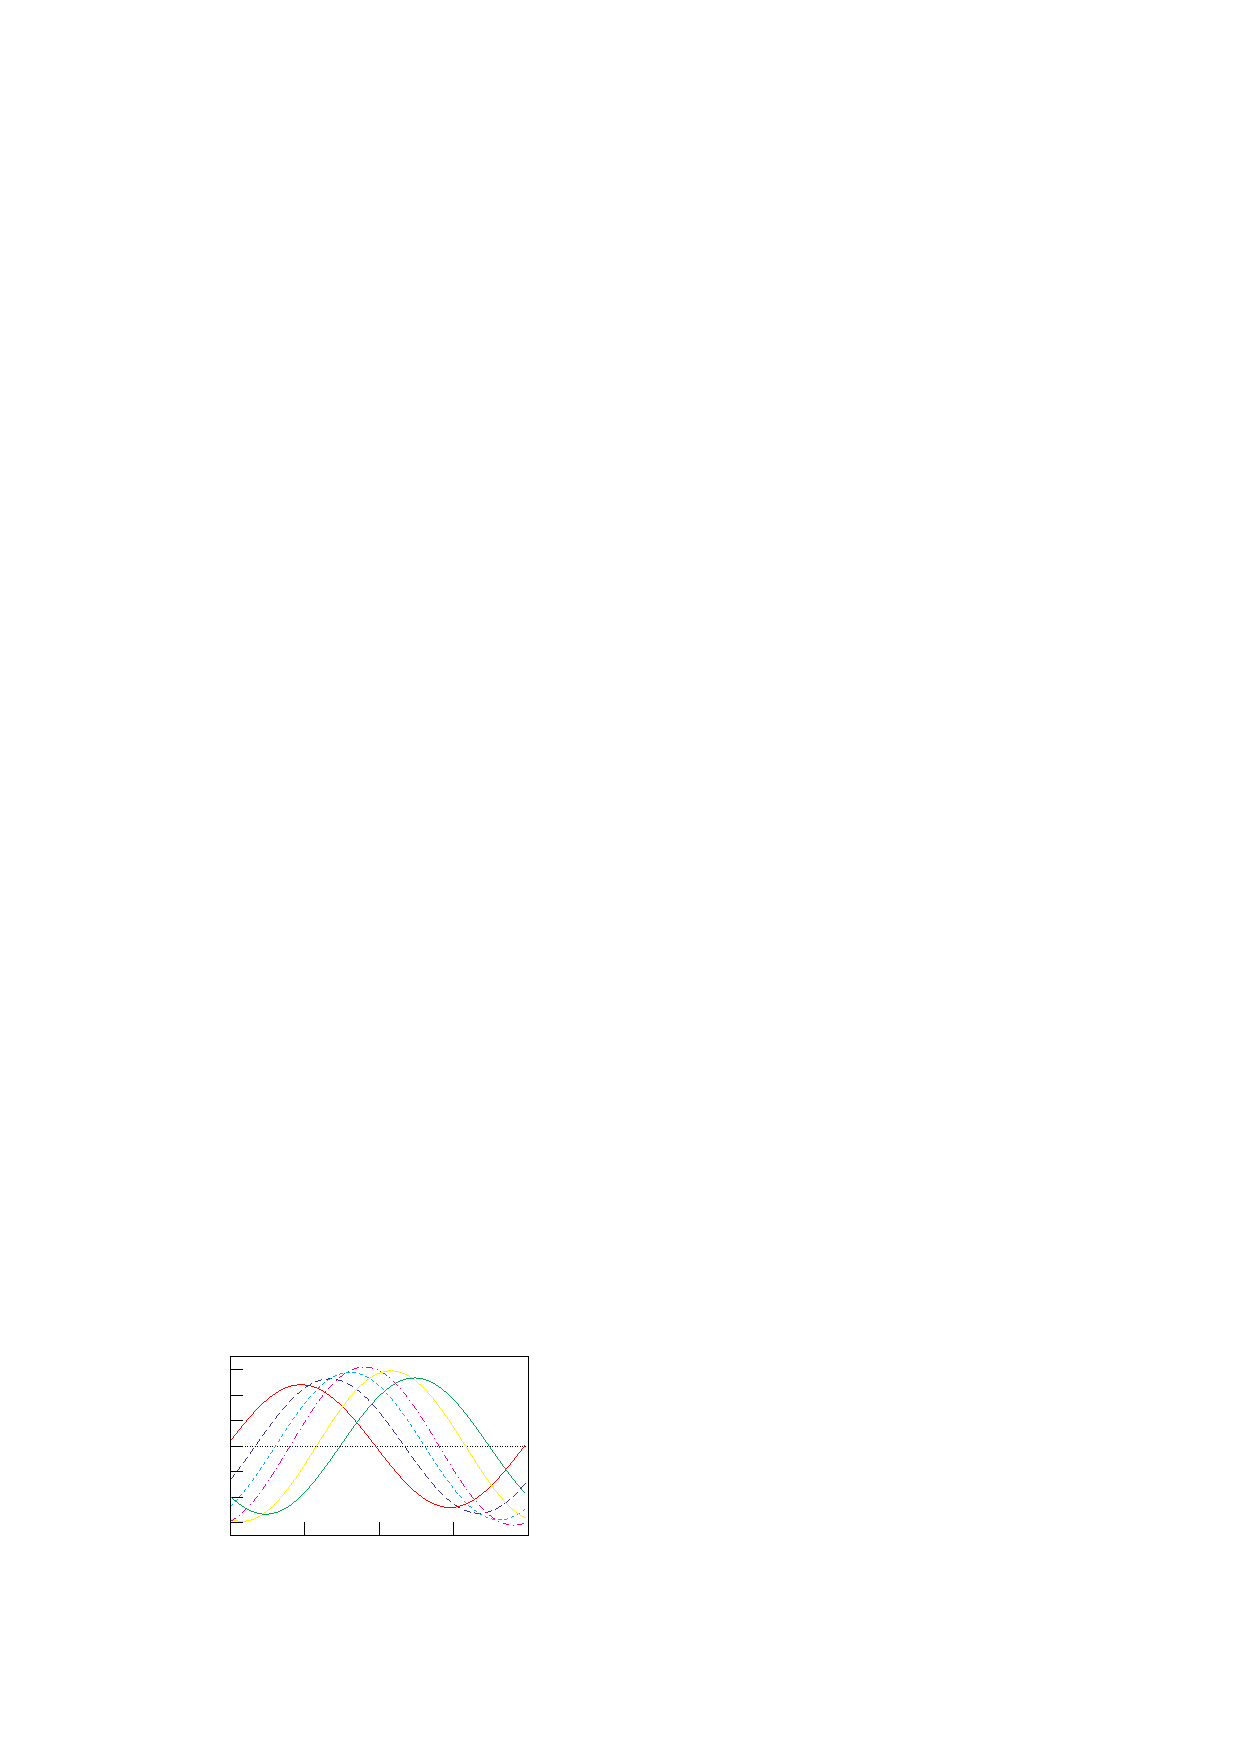
\includegraphics{Images/epslatex/Mel_ext_2}%
\end{picture}%
\begingroup
\setlength{\unitlength}{0.0200bp}%
\begin{picture}(9900,6480)(0,0)%
\put(1650,5624){\makebox(0,0)[r]{\strut{} 3}}%
\put(1650,5013){\makebox(0,0)[r]{\strut{} 2}}%
\put(1650,4401){\makebox(0,0)[r]{\strut{} 1}}%
\put(1650,3790){\makebox(0,0)[r]{\strut{} 0}}%
\put(1650,3179){\makebox(0,0)[r]{\strut{}-1}}%
\put(1650,2567){\makebox(0,0)[r]{\strut{}-2}}%
\put(1650,1956){\makebox(0,0)[r]{\strut{}-3}}%
\put(9075,1100){\makebox(0,0){\strut{}$2\pi$}}%
\put(7287,1100){\makebox(0,0){\strut{}$3\pi\slash{2}$}}%
\put(5500,1100){\makebox(0,0){\strut{}$\pi$}}%
\put(3713,1100){\makebox(0,0){\strut{}${\pi}\slash{2}$}}%
\put(1925,1100){\makebox(0,0){\strut{}0}}%
\put(550,3790){\rotatebox{90}{\makebox(0,0){\strut{}$\mathcal{M}^{\left(1\right)}_{h}\left(\psi_{0}\right)$}}}%
\put(5500,275){\makebox(0,0){\strut{}$\psi_0$}}%
\end{picture}%
\endgroup
\endinput
 \label{fig:Mel_ext_2} }
\end{center}
\caption[Mel'nikov integrals for extensible rods in a magnetic field]{Mel'nikov integrals evaluate at homoclinic energy level where $B=1$, subfigure~\ref{fig:Mel_ext_1} displays a functions at a differing degrees of extensibility, as $(1\slash{J}-1\slash{K})$ ranges from $0.1$ to $0.2$ in increments of $0.02$. In subfigure~\ref{fig:Mel_ext_1} the Casimir $C_{2}$ varies from $1$ up to $2$ in increments of $0.2$.}
\label{fig:Mel_ext}
\end{figure}
% 
\par
By Mel'nikov's theorem~\ref{thm:melnikov} and its corollary~\ref{cor:melnikov} the system is no longer completely integrable if extensible. The transversal intersection of the unstable and unstable manifolds lead to Smale horseshoes on the Poincar\'e section of the homoclinic energy level. This phenonema is illustrated in figures~\ref{fig:poincare} and~\ref{fig:poincare_all} which clearly show the breakup of integrability into the typical plots, referred to as stochastic layers in~\cite{Guckenheimer83}, associated with the Poincar\'e-Birkhoff theorem. 
%
\begin{figure}[h!tb]
\begin{center}
\subfigure[][$\lambda=0.50$]{ \input{Images/epslatex/poincare_0.50.tex} \label{fig:poincare_0.50} }
\subfigure[][$\lambda=3.50$]{ \input{Images/epslatex/poincare_3.50.tex} \label{fig:poincare_3.50} }
\subfigure[][$\lambda=3.75$]{ \input{Images/epslatex/poincare_3.75.tex} \label{fig:poincare_3.75} }
\subfigure[][$\lambda=4.00$]{ %GNUPLOT: LaTeX picture with Postscript
\begin{picture}(0,0)%
\includegraphics{Images/epslatex/poincare_4.00.eps}%
\end{picture}%
\begingroup
\setlength{\unitlength}{0.0200bp}%
\begin{picture}(9900,6750)(0,0)%
\put(2200,1650){\makebox(0,0)[r]{\strut{}-2.5}}%
\put(2200,2105){\makebox(0,0)[r]{\strut{}-2}}%
\put(2200,2560){\makebox(0,0)[r]{\strut{}-1.5}}%
\put(2200,3015){\makebox(0,0)[r]{\strut{}-1}}%
\put(2200,3470){\makebox(0,0)[r]{\strut{}-0.5}}%
\put(2200,3925){\makebox(0,0)[r]{\strut{} 0}}%
\put(2200,4380){\makebox(0,0)[r]{\strut{} 0.5}}%
\put(2200,4835){\makebox(0,0)[r]{\strut{} 1}}%
\put(2200,5290){\makebox(0,0)[r]{\strut{} 1.5}}%
\put(2200,5745){\makebox(0,0)[r]{\strut{} 2}}%
\put(2200,6200){\makebox(0,0)[r]{\strut{} 2.5}}%
\put(2475,1100){\makebox(0,0){\strut{}-2.5}}%
\put(3795,1100){\makebox(0,0){\strut{}-2}}%
\put(5115,1100){\makebox(0,0){\strut{}-1.5}}%
\put(6435,1100){\makebox(0,0){\strut{}-1}}%
\put(7755,1100){\makebox(0,0){\strut{}-0.5}}%
\put(9075,1100){\makebox(0,0){\strut{} 0}}%
\put(550,3925){\rotatebox{90}{\makebox(0,0){\strut{}$p_{\theta}^{}$}}}%
\put(5775,275){\makebox(0,0){\strut{}$\theta$}}%
\end{picture}%
\endgroup
\endinput
 \label{fig:poincare_4.00} }
\end{center}
\caption[Poincar\'e sections of an extensible rod in a magnetic field on the homoclinic energy level]{\baselineskip=1.0\normalbaselineskip% 
Poincar\'e sections on the homoclinic energy level $h=1.109756$ for varying levels of $\lambda$ at the section determined by $\cos\psi=-0.95$. The Casimirs are $C_{1}=C_{2}=C_{3}=1$, the bending stiffness $B=1$, the torsional stiffness $C=4\slash3$, the applied moment is $M=1.70$ and the compressive stiffnesses are $J=1$, $K=50\slash41$.}
\label{fig:poincare}
\end{figure}
% 
\begin{figure}[h!tb]
\begin{center}
%GNUPLOT: LaTeX picture with Postscript
\begin{picture}(0,0)%
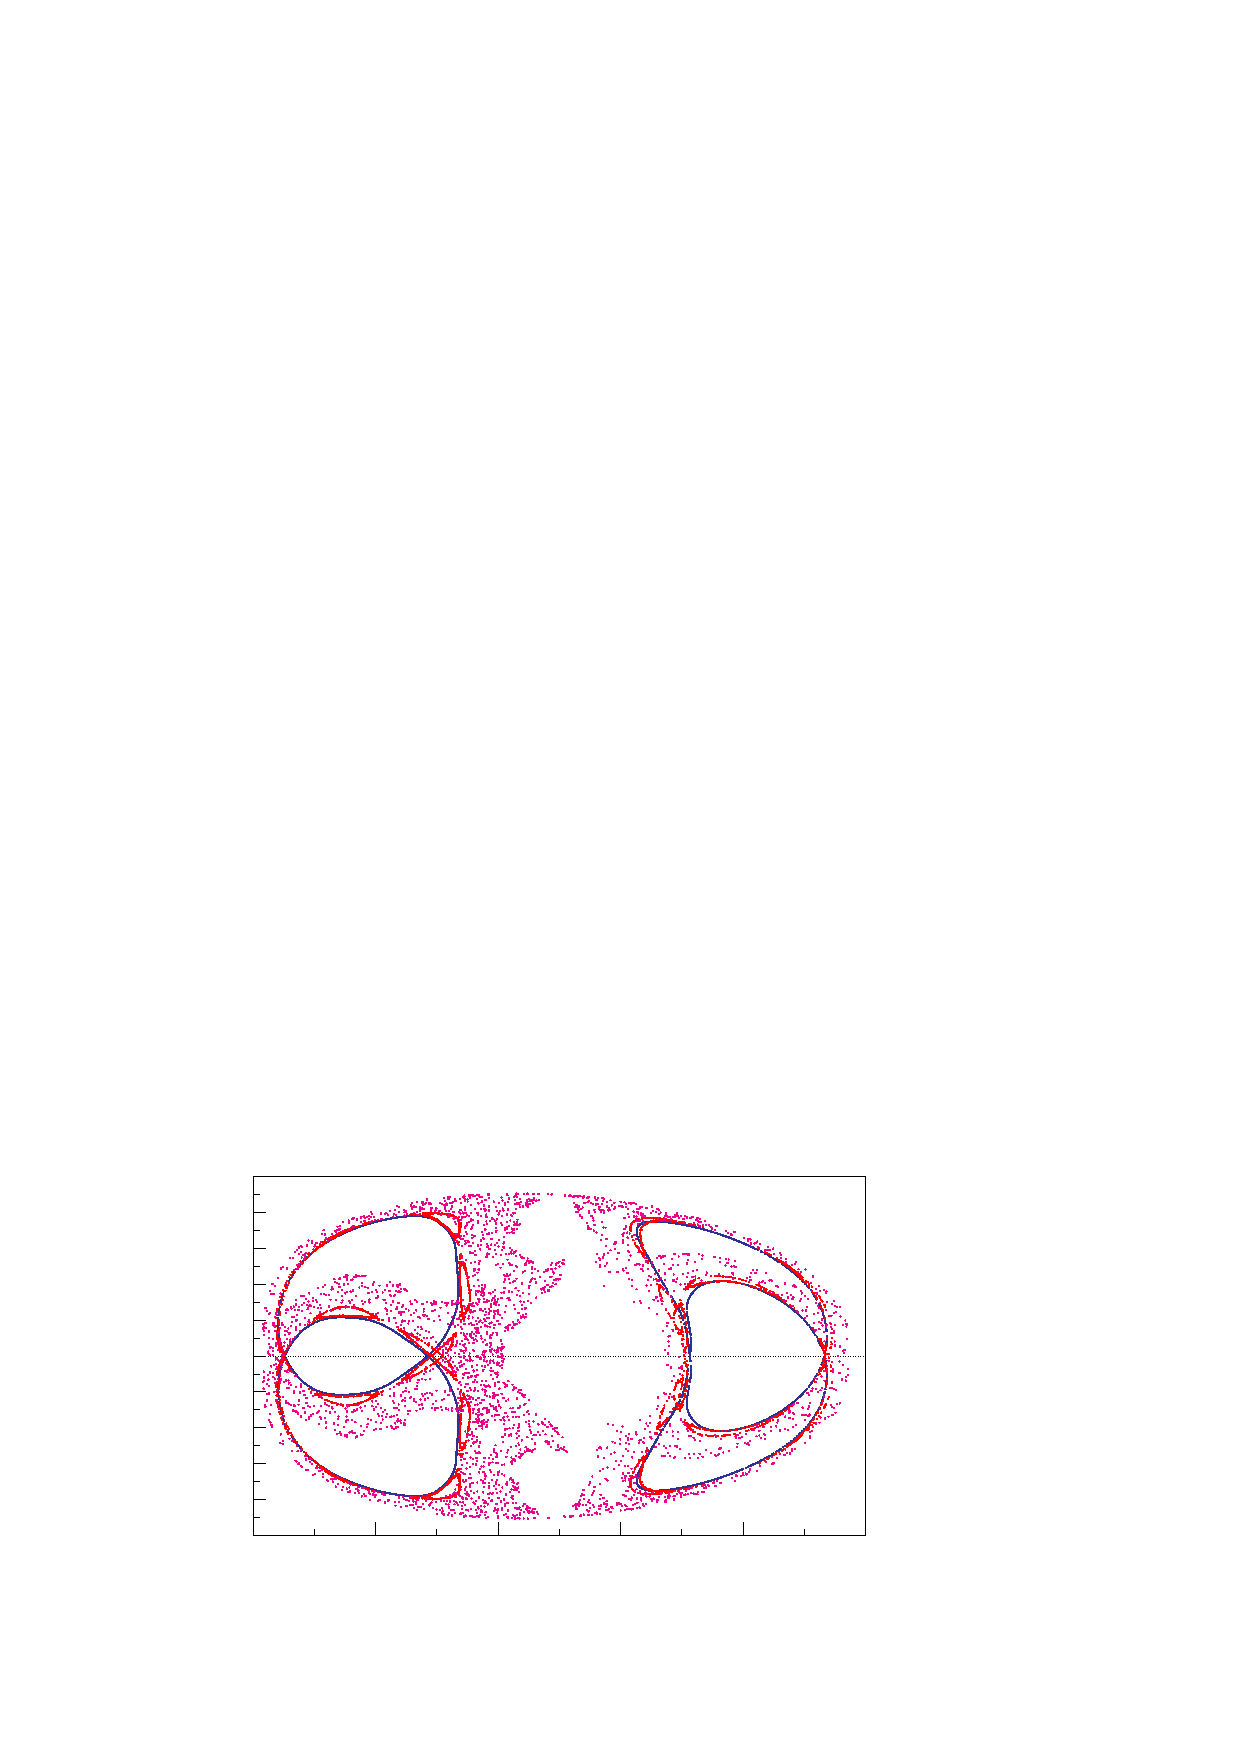
\includegraphics{Images/epslatex/poincare_all}%
\end{picture}%
\begingroup
\setlength{\unitlength}{0.0200bp}%
\begin{picture}(18000,10800)(0,0)%
\put(2200,1650){\makebox(0,0)[r]{\strut{}-2.5}}%
\put(2200,2510){\makebox(0,0)[r]{\strut{}-2}}%
\put(2200,3370){\makebox(0,0)[r]{\strut{}-1.5}}%
\put(2200,4230){\makebox(0,0)[r]{\strut{}-1}}%
\put(2200,5090){\makebox(0,0)[r]{\strut{}-0.5}}%
\put(2200,5950){\makebox(0,0)[r]{\strut{} 0}}%
\put(2200,6810){\makebox(0,0)[r]{\strut{} 0.5}}%
\put(2200,7670){\makebox(0,0)[r]{\strut{} 1}}%
\put(2200,8530){\makebox(0,0)[r]{\strut{} 1.5}}%
\put(2200,9390){\makebox(0,0)[r]{\strut{} 2}}%
\put(2200,10250){\makebox(0,0)[r]{\strut{} 2.5}}%
\put(2475,1100){\makebox(0,0){\strut{}-2.5}}%
\put(5415,1100){\makebox(0,0){\strut{}-2}}%
\put(8355,1100){\makebox(0,0){\strut{}-1.5}}%
\put(11295,1100){\makebox(0,0){\strut{}-1}}%
\put(14235,1100){\makebox(0,0){\strut{}-0.5}}%
\put(17175,1100){\makebox(0,0){\strut{} 0}}%
\put(550,5950){\rotatebox{90}{\makebox(0,0){\strut{}$p_{\theta}^{}$}}}%
\put(9825,275){\makebox(0,0){\strut{}$\theta$}}%
\end{picture}%
\endgroup
\endinput

\end{center}
\caption[Poincar\'e sections of an extensible rod in a magnetic field on the homoclinic energy level at various $\lambda$]{\baselineskip=1.0\normalbaselineskip% 
Poincar\'e sections on the homoclinic energy level $h=1.109756$ for varying levels of $\lambda$ at the section determined by $\cos\psi=-0.95$ showing the collapse of the integrable structure. The Casimirs are $C_{1}=C_{2}=C_{3}=1$, the bending stiffness $B=1$, the torsional stiffness $C=4\slash3$, the applied moment is $M=1.70$ and the compressive stiffnesses are $J=1$, $K=50\slash41$. The projection at $\lambda=3.50$ is in dark blue, $\lambda=3.75$ in red and $\lambda=4.00$ in purple.}
\label{fig:poincare_all} 
\end{figure}